\documentclass[tikz,border=8pt]{standalone}
\usepackage{amsmath,amssymb}
\usepackage{tikz}
\usetikzlibrary{angles,quotes,calc}

\begin{document}
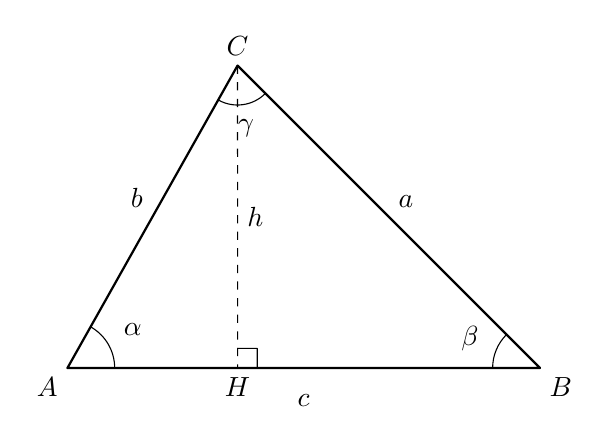
\begin{tikzpicture}[scale=1.2, line join=round]
  \coordinate (A) at (0,0);
  \coordinate (B) at (5,0);
  \coordinate (C) at (1.8,3.2);
  \coordinate (H) at ($(A)!(C)!(B)$);

  \draw[thick] (A) -- (B) -- (C) -- cycle;
  \draw[dashed] (C) -- (H);
  \pic[draw, angle radius=2.5mm] {right angle = C--H--B};

  \pic[draw, "$\alpha$", angle eccentricity=1.6, angle radius=6mm] {angle = B--A--C};
  \pic[draw, "$\beta$",  angle eccentricity=1.6, angle radius=6mm] {angle = C--B--A};
  \pic[draw, "$\gamma$", angle eccentricity=1.6, angle radius=5mm] {angle = A--C--B};

  \node[below left]  at (A) {$A$};
  \node[below right] at (B) {$B$};
  \node[above]       at (C) {$C$};
  \node[below]       at (H) {$H$};

  \path (A) -- (B) node[midway, below=6pt] {$c$};
  \path (B) -- (C) node[midway, above right] {$a$};
  \path (A) -- (C) node[midway, above left] {$b$};
  \path (C) -- (H) node[midway, right] {$h$};
\end{tikzpicture}
\end{document}
